\documentclass{summarysheet}

\begin{document}


\maketitle{2}{The Electric Field I}


\begin{topicbox}{The Electric Field Concept}

\begin{multicols}{2}

\noindent The electric field is an alteration of space surrounding charge. It is created by source charge and exerts an electric force on other charge.

The electric field is defined by its effect on a \emph{test charge} $q$:
\[
\vec{E} = \frac{\vec{F}_\text{on $q$}}{q}.
\]

The units of the electric field are N/C or V/m.

We can visualize the electric field through \emph{electric field lines}:
\begin{itemize}
\item The field direction is tangent to the curve at each point.
\item Lines closer together indicate stronger electric fields.
\item Field lines start on positive charge and end on negative.
\item Field lines never cross.
\end{itemize}


\begin{center}
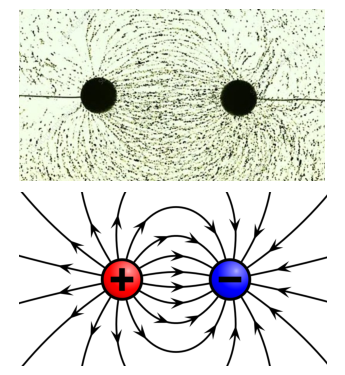
\includegraphics[scale=1]{fig_lines.pdf}
\end{center}

\end{multicols}

\end{topicbox}

\begin{multicols}{2}

\begin{topicbox}{A Single Point Charge}

\noindent A single point charge $q$ generates an electric field given by
\begin{teqbox}
\[
\vec{E} = \frac{1}{4\pi \varepsilon_0 } \frac{q}{r^2} \, \hat{r}.
\]
\end{teqbox}

\begin{center}
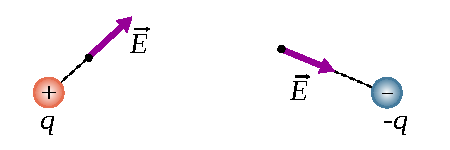
\includegraphics[scale=0.7]{fig_points.pdf}
\end{center}

The electric field points \emph{away} from positive charge and \emph{toward} negative charge.

\end{topicbox}


\begin{topicbox}{The Unit Vector $\hat{r}$}

\noindent We can specify the direction of the electric field by using the unit vector $\hat{r}$, which, like $\hat{i}$, $\hat{j}$, and $\hat{k}$, has no units and a magnitude equal to 1. Its only job is to point outward from the origin (where the charge is). Note that $-\hat{r}$, which would result if the point charge was negative, would then point toward the origin.

\begin{center}
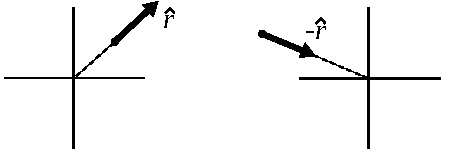
\includegraphics[scale=0.7]{fig_hat.pdf}
\end{center}


\end{topicbox}


\begin{topicbox}{Multiple Point Charges}

\noindent Multiple point charges $q_i$ generate an electric field given by the principle of superposition -- we just add up each individual electric field:
\begin{teqbox}
\[
\vec{E}_\text{net} = \sum_i \frac{1}{4\pi \varepsilon_0 } \frac{q_i}{r_i^2} \, \hat{r}_i.
\]
\end{teqbox}

\end{topicbox}

\begin{topicbox}{Charge Densities}

\noindent For extended charged objects, we can define three charge densities depending on the shape:
\begin{teqbox}
\begin{itemize}
\item Linear charge density (C/m):  $\lambda = Q/L$.
\item Surface charge density (C/m$^2$): $\eta = Q/A$.
\item Volume charge density (C/m$^3$): $\rho = Q/V$.
\end{itemize}
\end{teqbox}

\end{topicbox}


\begin{topicbox}{Continuous Charge Distributions}

\noindent If an extended object contains many excess electrons or protons we can consider the charge to be continuous rather than at a point. To calculate the electric field, we use the principle of superposition:
\begin{enumerate}
\item Divide the total charge $Q$ of the object into many small charges $dQ$, each of which acts like a point charge.
\item Find the electric field $d\vec{E}$ of each small charge $dQ$:
\[
d\vec{E} = \frac{1}{4 \pi \epsilon_0} \frac{dQ}{r^2} \, \hat{r}.
\]
\item Add all electric fields $d\vec{E}$ together by integrating over the object to find the net electric field $\vec{E}$.
\end{enumerate}

\begin{center}
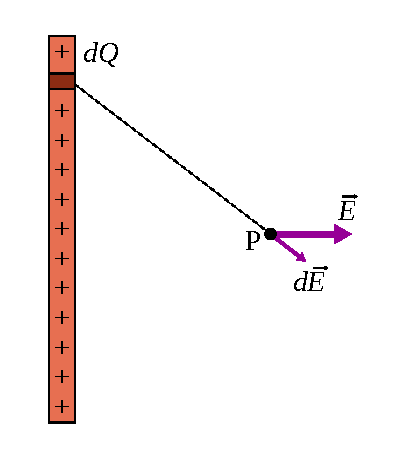
\includegraphics[scale=0.7]{fig_continuous.pdf}
\end{center}


\end{topicbox}



\end{multicols}


\makebanner{Electricity and Magnetism}

\end{document}



